% Note that depending on your settings in the table of contents, subsections and subsubsections might appear virtually identical.
% Make sure to set the ToC depth and the numbering depth in the ToC the way you want.
\chapter{Methods}\label{ch:methods}
In this chapter, we describe the theory behind Retention based autoregressive models and methods for training retention based models. 
\section{Motivation}

To model conditional distributions defined in eq(2.4) exactly, we require a method that can process sequences of variable input length. In the realm of neural spiking data, which is frequently recorded at a sampling rate expressed in kHz, we require a method that can efficiently scale with the length of the sequence Furthermore, the patterns of neural activity increase exponentially with respect to the number of neurons, and hence the number of discrete tokens required to represent neural spike pattern at time step $t$ can be prohibitively large. For instance, if we are recording spike signals from $100$ neurons, in total there are $2^{100}$ possible firing patterns. Existing Transformer based models cannot be directly applied to model conditional distributions of these kind, without placing an assumption on the nature of probability distribution. \\

To address these challenges, we introduce "Retention", a mathematical operation to map a sequence of vectors $\{x_i\}_{i=1}^N$ to real valued vector $\zeta_i$ of same dimension. Retention is inspired from Score-life programming \cite{muraleedharan2023beyond}, a novel method to solve sequential decision making problems. In Score-life programming \cite{muraleedharan2023beyond}, Muraleedharan et.al applied the insight that the binary expansion of a real number can be used to represent a sequence of discrete variables. After constructing the mapping between a sequence of discrete variables and real numbers in a bounded interval, functions can be directly defined on the real numbers. By defining functions using this approach, we can model non-trivial relationships between elements of a sequence. In prior work \cite{muraleedharan2023beyond}, has showed that such functions have unique properties, which can be exploited in developing efficient methods for solving determinisitic reinforcement learning problems. In our work, we extend this insight to vector valued variables, which are typically encountered in deep learning settings. 

\section{Retention}
Mathematically, retention is defined as an exponentially weighted sum of a sequence of discrete vectors. If the vectors are drawn from a continuous space, then we perform thresholding operation to discretize the vectors. 
Specifically, given a sequence of vectors $\{x_i\}_{i=1}^N$, $x_i \in \mathbb{R}^d$ , Retention variable $ \zeta_k \in [0,1)^d$ as:

\begin{equation}
    \zeta_k = \sum_{j=1}^{k} 2^{- (\log M)j} \sum_{i=0}^{M-1} \sigma(w_i \otimes x_{k-j+1} + b_i)
\end{equation}


Here, $w_i, b_i \in \mathbb{R}^d$ are trainable parameters for the thresholding operation defined in inner summation. Given a vector $x_i \in \mathbb{R}^d$ as input, the inner summation operation acts like a smoothened step function, essentially discretizing elements of the vector to discrete values in the set: $\{0,1,2,,,M-1\}$. The outer summation operation, with an exponentially decaying factor maps the sequence of discrete vectors to a continuous real valued vector $\zeta_k$. If the input data is discrete, or binary as in the case of neural spike signals, then the thresholding operation can be omitted, and the retention variable can be defined as: 
\begin{equation}
    \zeta_i = \sum_{k=1}^{i-1} 2^{-k} (x_{i-k}) 
\end{equation}
Given a sequence of discrete vectors $\{x_i\}_{i=1}^N$, retention variable $\zeta_i$ stores the discrete vectors in the binary expansion of $\zeta_i$. If the vectors  $\{x_i\}_{i=1}^N$ are continuous, then we perform a thresholding operation first to discretize the vectors and perform discounted sum of these discretized vectors. \\

Retention can also be defined for sequence of matrices $\{\mathbf{X}_i\}_{i=1}^N$ as:

\begin{equation}
    \mathbf{\zeta}_k = \sum_{j=1}^{k} 2^{- (\log M)j} \sum_{i=0}^{M-1} \sigma(\mathbf{W}_i \otimes \mathbf{X}_{k-j+1} + \mathbf{B}_i)
\end{equation}

\subsection{Modelling Conditional Distributions with Retention Variables}
Now, we can approximate the conditional distribution defined in eq(3) using retention variables. Specifically, the product of conditional distributions can now be approximated as:
\begin{equation}
   \prod_{i=1}^{N} p_d(\{x_{i}\}| \{x_1\},\{x_2\},..\{x_{i-1}\}) 
   \approx  \prod_{i=1}^{N} p_r(\{x_{i}\}|\zeta_i)
\end{equation}
In this case, sequence of vectors $\{x_j\}_{j=1}^i$ is encoded in the binary representation of Retention variable $\zeta_i$. Note that in this approach, a sequence of arbitrary length can be encoded within binary representation of $\zeta_i$. 
\subsection{Generative Models for neural spiking data}
Now, we apply Retention for generative modelling of neural spike patterns. Let $x_i \in \mathbb{R^d}$ denote the recording data from $d$ neurons at time step $i$. To learn the dynamics of the brain from neural recordings in an unsupervised manner, we maximize the following likelihood:
\begin{equation}
    \mathcal{L}(X,\theta) = -\sum_i log(p_r(\{x_{i}\}|\zeta_i;\theta))
\end{equation}
Here, $X = \{x_1,x_2,....x_M\}$, is the dataset of neural recordings. \\

Note that in this approach, the context window is not bounded, and the complexity of learning the parametrized model $p_r(\{x_{i}\}|\zeta_i;\theta)$ is independent of the length of the context window.
 \\

 \subsection{Neural Spike to behavior model }

 To learn the correlation between neural dynamics and behavior, we follow a similar approach and approximate the conditional distribution defined in eq(2.4) with:
\\
 \begin{equation}
   \prod_{i=1}^{N} p_b(\{y_{i}\}| \{x_1\},\{x_2\},..\{x_{i-1}\}) 
   \approx  \prod_{i=1}^{N} p_b(\{y_{i}\}|\zeta_i)
\end{equation}
We define the loss function associated with this approach as the negative log-likelihood of the observed behavioral outcomes given the estimated neural activity states. Formally, the loss function \( \mathcal{L} \) is expressed as:

\[
\mathcal{L}(X,Y,\phi) = -\sum_{i} \log p_b(\{y_i\}|\zeta_i;\phi)
\]

We further assume that the conditional distribution is of the form:

\begin{equation}
p_b(\{y_i\}|\zeta_i;\phi) = \mathbf{\mathcal{N}}(f_b(\zeta_i;\phi), \sigma^2 I_d)
\end{equation}
After this assumption the loss function takes the form of Mean Squared Error loss given by:
\begin{equation}
    \mathcal{L}(X,\theta) = -\sum_i ||f_b(\zeta_i;\phi) - y_i||_2
\end{equation}
\section{Architecture}

For predicting neural dynamics and inferring behavior given spike data, we employ a convolutional network based on the UNet architecture \cite{ronneberger2015u}. The UNet model has proven to be highly effective in various image segmentation tasks and is well-suited for our objective of decoding neural activity.

Our architecture comprises multiple key components designed to handle the intricacies of spike data and capture the underlying patterns in neural dynamics. The UNet structure consists of an encoder and decoder network, facilitating the extraction and reconstruction of features at different abstraction levels. This enables the model to learn hierarchical representations of the spatio-temporal input data, enhancing its ability to discern complex relationships within the neural activity.

For the autoregressive model, we use a standard UNet model with retention variable $\zeta_k$ at input layer. In our implementation, we computed the retention variable $\zeta_k$ online, during training. Intuitively, given a sequence of black and white images that represent neural firing patterns at various time steps, the retention layer convert the sequence of black and white images to a single grayscale image, which is then fed into the UNet architecture. Each pixel in the image correspond to a neuron or unit from which the neural spiking data is collected. 
In a typical UNet model employed for medical image segmentation tasks, the output layer predicts the masked image corresponding to the input image. In our case, the output layer predicts the probability of different neurons firing at the next timestep. Since the UNet model is a fully convolutional network, the model can be trained on diverse set of input datasets, consisting of variable number of input neurons. Hence, we can utilize the architecture on learning from a large dataset of neural recordings collected using various experimental setups.  \\



\begin{figure}
  \centering
  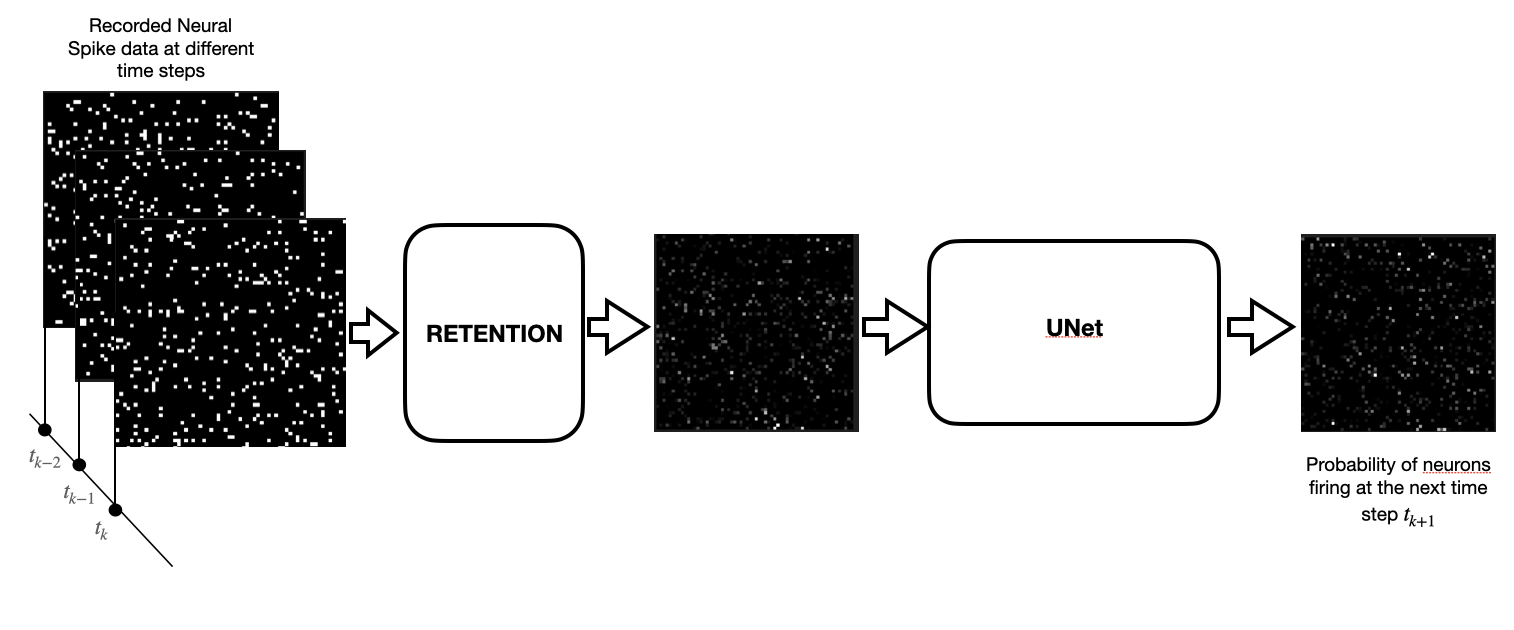
\includegraphics[width=1.0\linewidth]{figures/retention_autoregressive.png}  
  \caption{Your Caption Here}
  \label{fig:your_label}  % You can use this label to refer to the figure in the text
\end{figure}
For predicting behaviour from observed neural spiking data, we add extra fully connected layers to the output of UNet model to predict the behaviour variable corresponding to input neural spiking data. 
For instance, if we are interested in modelling the dynamics of human motor cortex and finding relationship between spike patterns in motor cortex and trajectory of finger motion, then our output layer should be three-dimensional to represent the three-dimensional motion of human finger. In addition to modelling kinematics of finger, the architecture can also be applied to other tasks such as predicting the probability of seizure given neural spike recordings. 


\begin{figure}
    \centering
    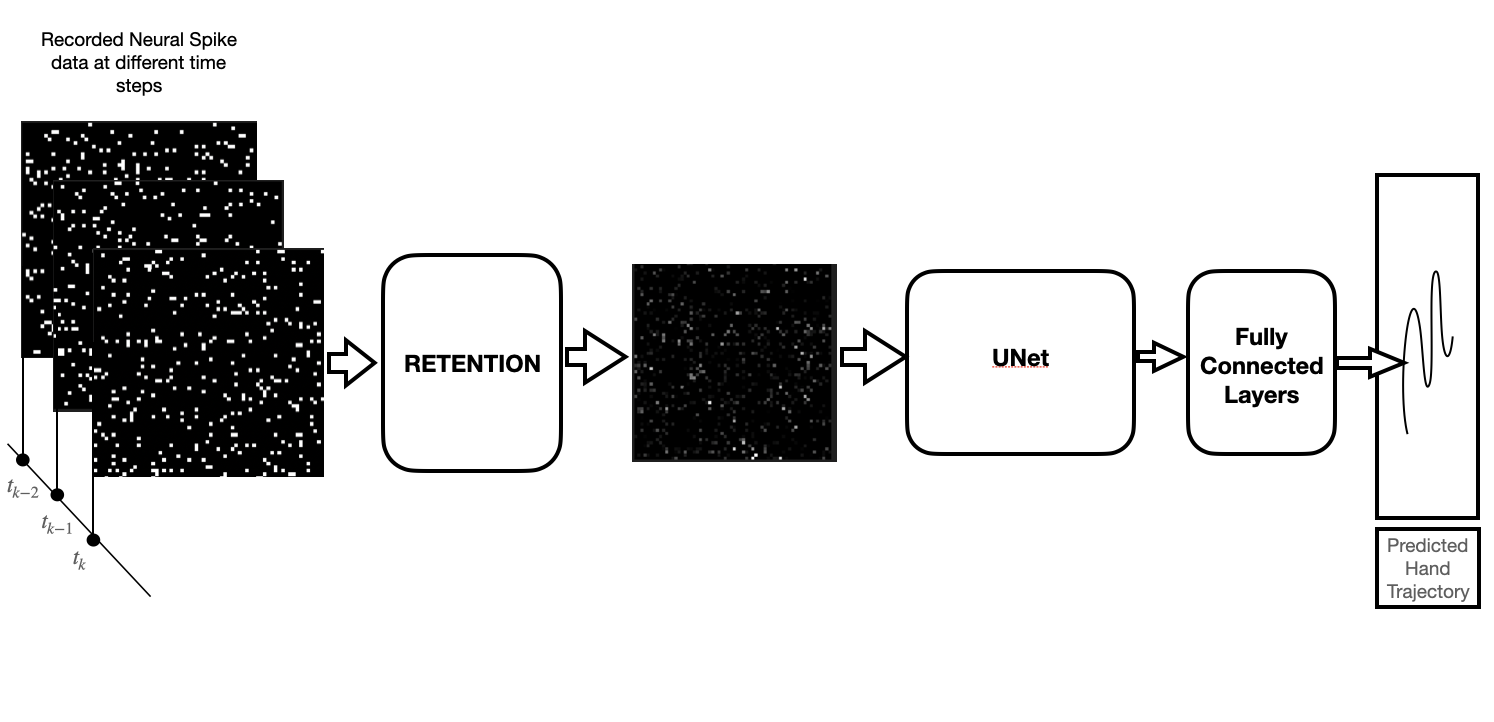
\includegraphics[width=1.0\linewidth]{figures/retention_spike_to_behavior.png}  
    \caption{Your Caption Here}
    \label{fig:your_label}  % You can use this label to refer to the figure in the text
  \end{figure}

\section{Training Retention Based Models}



\begin{algorithm}
    \caption{Training Algorithm for Image Classification}
    \begin{algorithmic}[1]
    \Procedure{TrainModel}{$Data$, $Epochs$}
        \State Initialize $Model$
        \For{$epoch = 1$ \textbf{to} $Epochs$}
            \For{each $batch$ in $Data$}
                \State $Inputs, Targets \gets batch$
                \State $Predictions \gets \Call{ForwardPass}{Model, Inputs}$
                \State $Loss \gets \Call{ComputeLoss}{Predictions, Targets}$
                \State Perform backpropagation to compute gradients
                \State Update $Model$ parameters
            \EndFor
            \State Evaluate model on validation data
            \If{performance improves}
                \State Update best model
            \EndIf
        \EndFor
        \State \textbf{return} Trained $Model$
    \EndProcedure
    \end{algorithmic}
    \end{algorithm}
    

In this section, we describe how retention based models are trained. 
While training the model, we apply eq(6) to recursively update $\zeta_i$ in an online fashion, instead of pre-computing and storing $\{\zeta_i\}_{i=1}^N$ separately

\subsection{Online Computation of Retention Variable}

\subsection{Offline Computation of Retention Variable}



